% Created by tikzDevice version 0.12.6 on 2026-05-29 08:00:27
% !TEX encoding = UTF-8 Unicode
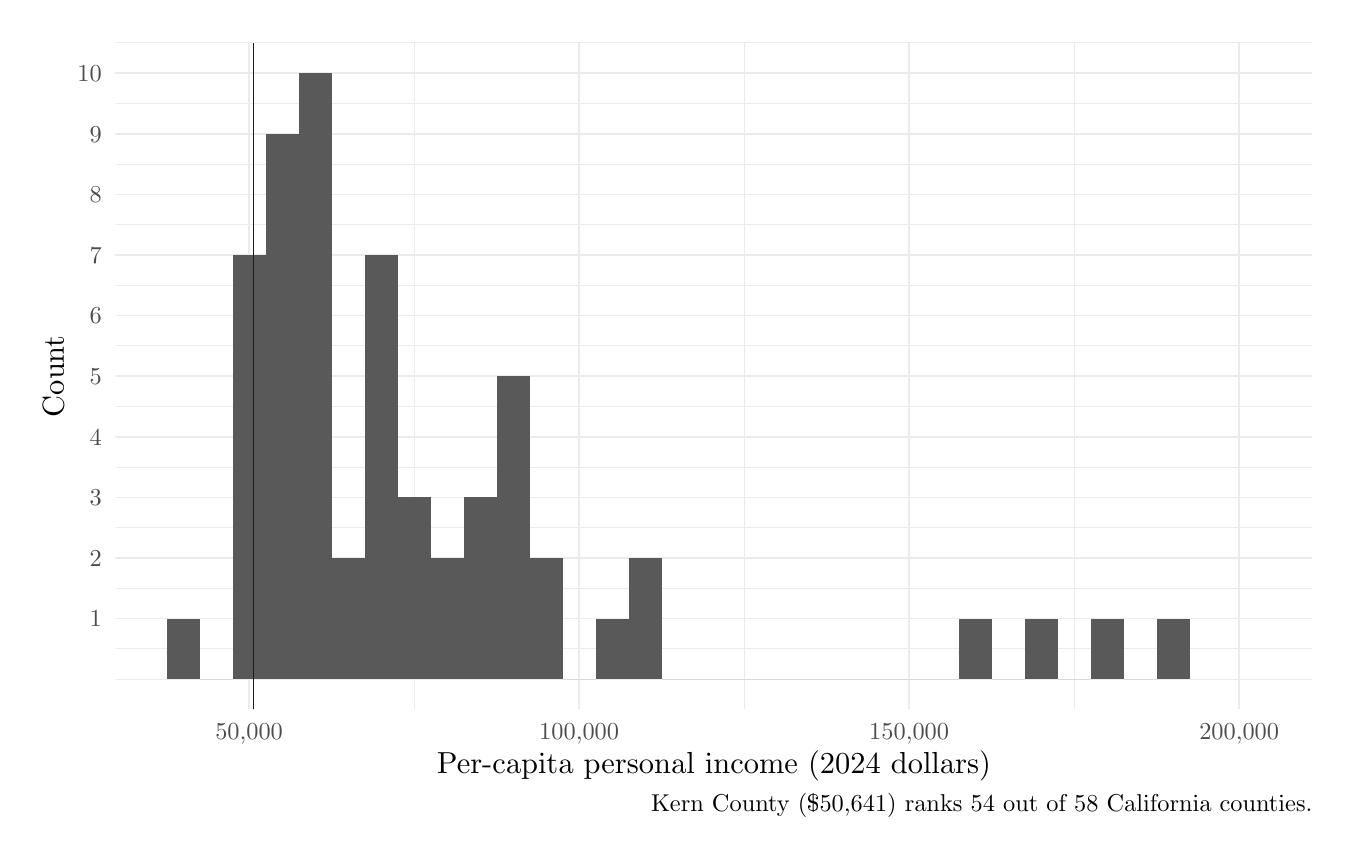
\begin{tikzpicture}[x=1pt,y=1pt]
\definecolor{fillColor}{RGB}{255,255,255}
\path[use as bounding box,fill=fillColor,fill opacity=0.00] (0,0) rectangle (469.75,290.32);
\begin{scope}
\path[clip] (  0.00,  0.00) rectangle (469.75,290.32);
\definecolor{fillColor}{RGB}{255,255,255}

\path[fill=fillColor] (  0.00,  0.00) rectangle (469.76,290.32);
\end{scope}
\begin{scope}
\path[clip] ( 31.71, 43.96) rectangle (464.25,284.82);
\definecolor{drawColor}{gray}{0.92}

\path[draw=drawColor,line width= 0.3pt,line join=round] ( 31.71, 54.91) --
	(464.25, 54.91);

\path[draw=drawColor,line width= 0.3pt,line join=round] ( 31.71, 65.85) --
	(464.25, 65.85);

\path[draw=drawColor,line width= 0.3pt,line join=round] ( 31.71, 87.75) --
	(464.25, 87.75);

\path[draw=drawColor,line width= 0.3pt,line join=round] ( 31.71,109.65) --
	(464.25,109.65);

\path[draw=drawColor,line width= 0.3pt,line join=round] ( 31.71,131.55) --
	(464.25,131.55);

\path[draw=drawColor,line width= 0.3pt,line join=round] ( 31.71,153.44) --
	(464.25,153.44);

\path[draw=drawColor,line width= 0.3pt,line join=round] ( 31.71,175.34) --
	(464.25,175.34);

\path[draw=drawColor,line width= 0.3pt,line join=round] ( 31.71,197.24) --
	(464.25,197.24);

\path[draw=drawColor,line width= 0.3pt,line join=round] ( 31.71,219.13) --
	(464.25,219.13);

\path[draw=drawColor,line width= 0.3pt,line join=round] ( 31.71,241.03) --
	(464.25,241.03);

\path[draw=drawColor,line width= 0.3pt,line join=round] ( 31.71,262.93) --
	(464.25,262.93);

\path[draw=drawColor,line width= 0.3pt,line join=round] ( 31.71,284.82) --
	(464.25,284.82);

\path[draw=drawColor,line width= 0.3pt,line join=round] (139.64, 43.96) --
	(139.64,284.82);

\path[draw=drawColor,line width= 0.3pt,line join=round] (258.90, 43.96) --
	(258.90,284.82);

\path[draw=drawColor,line width= 0.3pt,line join=round] (378.15, 43.96) --
	(378.15,284.82);

\path[draw=drawColor,line width= 0.6pt,line join=round] ( 31.71, 76.80) --
	(464.25, 76.80);

\path[draw=drawColor,line width= 0.6pt,line join=round] ( 31.71, 98.70) --
	(464.25, 98.70);

\path[draw=drawColor,line width= 0.6pt,line join=round] ( 31.71,120.60) --
	(464.25,120.60);

\path[draw=drawColor,line width= 0.6pt,line join=round] ( 31.71,142.49) --
	(464.25,142.49);

\path[draw=drawColor,line width= 0.6pt,line join=round] ( 31.71,164.39) --
	(464.25,164.39);

\path[draw=drawColor,line width= 0.6pt,line join=round] ( 31.71,186.29) --
	(464.25,186.29);

\path[draw=drawColor,line width= 0.6pt,line join=round] ( 31.71,208.18) --
	(464.25,208.18);

\path[draw=drawColor,line width= 0.6pt,line join=round] ( 31.71,230.08) --
	(464.25,230.08);

\path[draw=drawColor,line width= 0.6pt,line join=round] ( 31.71,251.98) --
	(464.25,251.98);

\path[draw=drawColor,line width= 0.6pt,line join=round] ( 31.71,273.88) --
	(464.25,273.88);

\path[draw=drawColor,line width= 0.6pt,line join=round] ( 80.01, 43.96) --
	( 80.01,284.82);

\path[draw=drawColor,line width= 0.6pt,line join=round] (199.27, 43.96) --
	(199.27,284.82);

\path[draw=drawColor,line width= 0.6pt,line join=round] (318.52, 43.96) --
	(318.52,284.82);

\path[draw=drawColor,line width= 0.6pt,line join=round] (437.78, 43.96) --
	(437.78,284.82);
\definecolor{fillColor}{gray}{0.35}

\path[fill=fillColor] ( 50.20, 54.91) rectangle ( 62.12, 76.80);

\path[fill=fillColor] ( 62.12, 54.91) rectangle ( 74.05, 54.91);

\path[fill=fillColor] ( 74.05, 54.91) rectangle ( 85.97,208.18);

\path[fill=fillColor] ( 85.97, 54.91) rectangle ( 97.90,251.98);

\path[fill=fillColor] ( 97.90, 54.91) rectangle (109.83,273.88);

\path[fill=fillColor] (109.83, 54.91) rectangle (121.75, 98.70);

\path[fill=fillColor] (121.75, 54.91) rectangle (133.68,208.18);

\path[fill=fillColor] (133.68, 54.91) rectangle (145.60,120.60);

\path[fill=fillColor] (145.60, 54.91) rectangle (157.53, 98.70);

\path[fill=fillColor] (157.53, 54.91) rectangle (169.45,120.60);

\path[fill=fillColor] (169.45, 54.91) rectangle (181.38,164.39);

\path[fill=fillColor] (181.38, 54.91) rectangle (193.30, 98.70);

\path[fill=fillColor] (193.30, 54.91) rectangle (205.23, 54.91);

\path[fill=fillColor] (205.23, 54.91) rectangle (217.16, 76.80);

\path[fill=fillColor] (217.16, 54.91) rectangle (229.08, 98.70);

\path[fill=fillColor] (229.08, 54.91) rectangle (241.01, 54.91);

\path[fill=fillColor] (241.01, 54.91) rectangle (252.93, 54.91);

\path[fill=fillColor] (252.93, 54.91) rectangle (264.86, 54.91);

\path[fill=fillColor] (264.86, 54.91) rectangle (276.78, 54.91);

\path[fill=fillColor] (276.78, 54.91) rectangle (288.71, 54.91);

\path[fill=fillColor] (288.71, 54.91) rectangle (300.64, 54.91);

\path[fill=fillColor] (300.64, 54.91) rectangle (312.56, 54.91);

\path[fill=fillColor] (312.56, 54.91) rectangle (324.49, 54.91);

\path[fill=fillColor] (324.49, 54.91) rectangle (336.41, 54.91);

\path[fill=fillColor] (336.41, 54.91) rectangle (348.34, 76.80);

\path[fill=fillColor] (348.34, 54.91) rectangle (360.26, 54.91);

\path[fill=fillColor] (360.26, 54.91) rectangle (372.19, 76.80);

\path[fill=fillColor] (372.19, 54.91) rectangle (384.11, 54.91);

\path[fill=fillColor] (384.11, 54.91) rectangle (396.04, 76.80);

\path[fill=fillColor] (396.04, 54.91) rectangle (407.97, 54.91);

\path[fill=fillColor] (407.97, 54.91) rectangle (419.89, 76.80);
\definecolor{drawColor}{RGB}{0,26,112}

\path[draw=drawColor,line width= 0.6pt,line join=round] ( 81.54, 43.96) -- ( 81.54,284.82);
\end{scope}
\begin{scope}
\path[clip] (  0.00,  0.00) rectangle (469.75,290.32);
\definecolor{drawColor}{gray}{0.30}

\node[text=drawColor,anchor=base east,inner sep=0pt, outer sep=0pt, scale=  0.88] at ( 26.76, 73.77) {1};

\node[text=drawColor,anchor=base east,inner sep=0pt, outer sep=0pt, scale=  0.88] at ( 26.76, 95.67) {2};

\node[text=drawColor,anchor=base east,inner sep=0pt, outer sep=0pt, scale=  0.88] at ( 26.76,117.57) {3};

\node[text=drawColor,anchor=base east,inner sep=0pt, outer sep=0pt, scale=  0.88] at ( 26.76,139.46) {4};

\node[text=drawColor,anchor=base east,inner sep=0pt, outer sep=0pt, scale=  0.88] at ( 26.76,161.36) {5};

\node[text=drawColor,anchor=base east,inner sep=0pt, outer sep=0pt, scale=  0.88] at ( 26.76,183.26) {6};

\node[text=drawColor,anchor=base east,inner sep=0pt, outer sep=0pt, scale=  0.88] at ( 26.76,205.15) {7};

\node[text=drawColor,anchor=base east,inner sep=0pt, outer sep=0pt, scale=  0.88] at ( 26.76,227.05) {8};

\node[text=drawColor,anchor=base east,inner sep=0pt, outer sep=0pt, scale=  0.88] at ( 26.76,248.95) {9};

\node[text=drawColor,anchor=base east,inner sep=0pt, outer sep=0pt, scale=  0.88] at ( 26.76,270.85) {10};
\end{scope}
\begin{scope}
\path[clip] (  0.00,  0.00) rectangle (469.75,290.32);
\definecolor{drawColor}{gray}{0.30}

\node[text=drawColor,anchor=base,inner sep=0pt, outer sep=0pt, scale=  0.88] at ( 80.01, 32.95) {50,000};

\node[text=drawColor,anchor=base,inner sep=0pt, outer sep=0pt, scale=  0.88] at (199.27, 32.95) {100,000};

\node[text=drawColor,anchor=base,inner sep=0pt, outer sep=0pt, scale=  0.88] at (318.52, 32.95) {150,000};

\node[text=drawColor,anchor=base,inner sep=0pt, outer sep=0pt, scale=  0.88] at (437.78, 32.95) {200,000};
\end{scope}
\begin{scope}
\path[clip] (  0.00,  0.00) rectangle (469.75,290.32);
\definecolor{drawColor}{RGB}{0,0,0}

\node[text=drawColor,anchor=base,inner sep=0pt, outer sep=0pt, scale=  1.10] at (247.98, 20.91) {Per-capita personal income (2024 dollars)};
\end{scope}
\begin{scope}
\path[clip] (  0.00,  0.00) rectangle (469.75,290.32);
\definecolor{drawColor}{RGB}{0,0,0}

\node[text=drawColor,rotate= 90.00,anchor=base,inner sep=0pt, outer sep=0pt, scale=  1.10] at ( 13.08,164.39) {Count};
\end{scope}
\begin{scope}
\path[clip] (  0.00,  0.00) rectangle (469.75,290.32);
\definecolor{drawColor}{RGB}{0,0,0}

\node[text=drawColor,anchor=base east,inner sep=0pt, outer sep=0pt, scale=  0.88] at (464.25,  7.21) {Kern County (\$50,641) ranks 54 out of 58 California counties.};
\end{scope}
\end{tikzpicture}
